\documentclass[aspectratio=1610,t]{beamer}

% Colors
\usepackage{color}
\definecolor{mainorange}{HTML}{EC811B}
\definecolor{lightgrey}{HTML}{888888}

% Syntax highlighting
\usepackage{minted}
\usepackage{alltt}
\newcommand\hi[1]{{\color{mainorange} \textbf{#1}}}

% Theme
\usetheme[%
	subsectionpage=progressbar,
	numbering=fraction,
	progressbar=foot,
]{metropolis}

% Customization
\setbeamertemplate{section in toc}[sections numbered]
\setbeamerfont{title}{size=\fontsize{30}{30}}
\setbeamerfont{block title}{size=\large}
\newcommand\sep{\textcolor{lightgrey}{\rule{\linewidth}{0.05mm}}}

% Meta
\title{Rust<T>}
\date{7. 9. 2016}
\author{Stefan Schindler (@dns2utf8)}
\institute{Coredump Rapperswil}

% Backgrounds
\pgfdeclareimage[width=\paperwidth]{bglight}{background-light.pdf}
\pgfdeclareimage[width=\paperwidth]{bgdark}{background-dark.pdf}
\pgfdeclareimage[width=\paperwidth]{bginverted}{background-inverted.pdf}

\begin{document}

{
\usebackgroundtemplate{\pgfuseimage{bgdark}}
\maketitle
}

% ----------------------------------------------------------------- %
\usebackgroundtemplate{\pgfuseimage{bglight}}
\begin{frame}[noframenumbering]
	\frametitle{Outline}
	\tableofcontents
\end{frame}

% ----------------------------------------------------------------- %

\usebackgroundtemplate{\pgfuseimage{bglight}}

{
\usebackgroundtemplate{\pgfuseimage{bgdark}}
\section{Admin}
}

\begin{frame}[fragile]{Admin}

\begin{itemize}
  \item Slides are online:
        \url{https://github.com/coredump-ch/rust-t}
  \item Examples are included in the \texttt{examples} directory.
  \item Slides of Danilo \& Raphael:
        \url{https://github.com/coredump-ch/intro-to-rust}
\end{itemize}

\end{frame}

{
\usebackgroundtemplate{\pgfuseimage{bgdark}}
\section{Recap from last time}
}

\begin{frame}[fragile]{Example 2: Generics}

\begin{minted}{rust}
fn min<T: Ord>(a: T, b: T) -> T {
    if a <= b { a } else { b }
}
\end{minted}
\pause
\begin{minted}{rust}
...

min(10i8,  20)    == 10;    // T is i8
min(10,    20u32) == 10;    // T is u32
min("abc", "xyz") == "abc"; // &str or Strings are Ord
min("abc".to_string(), "ABC".into()) == "ABC";

min(10i32, "xyz"); // error: mismatched types
\end{minted}

\end{frame}

{
\usebackgroundtemplate{\pgfuseimage{bgdark}}
\section{Simple Generics}
}
\begin{frame}[fragile]{Enum}
\begin{minted}{rust}
enum Colors {
  Red,
  Green,
  Blue,
}
use Colors::*;

fn draw(color: Colors) {
  match color {
    ...
  }
}
\end{minted}
\end{frame}

\begin{frame}[fragile]{Enum}
\begin{minted}{rust}
use Colors::*;

fn main() {
  draw(Red);
  draw(Blue);
}

fn draw(color: Colors) {
  match color {
    Red   => 0xff0000,
    Green => 0x00ff00,
    Blue  => 0x0000ff,
  }; // no return
}
\end{minted}
\end{frame}


\begin{frame}[fragile]{Enum: non-exhaustive patterns}
\begin{minted}{rust}
fn draw(color: Colors) {
  match color {
    Red => 0xff0000,
    // Green => 0x00ff00,
    Blue => 0x0000ff,
  };
}
\end{minted}
\end{frame}
% \pause
% error: non-exhaustive patterns: `Green` not covered [E0004]

\begin{frame}[fragile]{Enum: non-exhaustive patterns}
\begin{minted}[breaklines=true]{sh}
$ cargo run
src/main.rs:15:3: 19:4 error: non-exhaustive patterns: `Green` not covered [E0004]
src/main.rs:15   match color {
src/main.rs:16     Red => 0xff0000,
src/main.rs:17     // Green => 0x00ff00,
src/main.rs:18     Blue => 0x0000ff,
src/main.rs:19   }; // no return
src/main.rs:15:3: 19:4 help: run `rustc --explain E0004` to see a detailed explanation
error: aborting due to previous error
error: Could not compile `enum`.

To learn more, run the command again with --verbose.
\end{minted}
\end{frame}

{
\usebackgroundtemplate{\pgfuseimage{bgdark}}
\section{Into() complex Type}
}

\begin{frame}[fragile]{Into() complex Type: Infrastructure}
\begin{minted}[breaklines=true]{rust}
#[derive(Debug, Clone)]
struct MyObject {
  is : Option<isize>,
  st : Option<String>,
}

impl Into<MyObject> for isize {
  fn into(self) -> MyObject {
    MyObject {
      is : Some(self),
      st : None,
    }
  }
}
\end{minted}
\end{frame}

\begin{frame}[fragile]{Into() complex Type: Infrastructure}
and the implementation for \texttt{String}:
\begin{minted}[breaklines=true]{rust}
impl Into<MyObject> for String {
  fn into(self) -> MyObject {
    MyObject {
      is : None,
      st : Some(self),
    }
  }
}
\end{minted}
\end{frame}


\begin{frame}[fragile]{Into\(\) complex Type: Usage}
  \begin{minted}[breaklines=true]{rust}
  let m0 = MyObject { is : Some(42), st : Some("Self Made".into()) };
  \end{minted}

\pause

  use with \texttt{isize}:
  \begin{minted}[breaklines=true]{rust}
  let m1 : MyObject = 23.into();
  \end{minted}

\pause

  with \texttt{to\_owned()} for \texttt{String}:
  \begin{minted}[breaklines=true]{rust}
  let m2 : MyObject = "Coredump.ch".to_owned().into();
  \end{minted}
\end{frame}




{
\usebackgroundtemplate{\pgfuseimage{bgdark}}
\section{Enum impl}
}

\begin{frame}[fragile]{Enum impl: Infrastructure}
\begin{minted}[breaklines=true]{rust}
impl Person {
  // A function which takes a `Person` enum as an argument
  // and returns nothing.
  fn inspect(self) {
    // Usage of an `enum` must cover all cases (irrefutable)
    // so a `match` is used to branch over it.
    match self {
      Person::Engineer => { ... },
      ...
    }
  }
}
\end{minted}
\end{frame}


\begin{frame}[fragile]{Enum impl: Usage}
if we have an \texttt{Enum}:
  \begin{minted}[breaklines=true]{rust}
  let rohan    = Person::Engineer;
  \end{minted}

%\pause
we can then use the method on the insance:
  \begin{minted}[breaklines=true]{rust}
  rohan.inspect();
  \end{minted}
\end{frame}




{
\usebackgroundtemplate{\pgfuseimage{bgdark}}
\section{Transport Data with Enums}
}

\begin{frame}[fragile]{Enum Transport: Infrastructure}
\begin{minted}[breaklines=true]{rust}
#[derive(Debug)]
enum CompoundIndex {
  SearchIsize(isize),
  SearchString(String),
}
use CompoundIndex::*;
\end{minted}
\end{frame}


\begin{frame}[fragile]{Enum Transport: Usage}
a number:
  \begin{minted}[breaklines=true]{rust}
  let number = SearchIsize(42);
  \end{minted}

\pause
a \texttt{String}:
  \begin{minted}[breaklines=true]{rust}
  let string = SearchString("Coredump.ch".into());
  \end{minted}

\pause
an empty \texttt{String}:
  \begin{minted}[breaklines=true]{rust}
  let string = SearchString("".into());
  \end{minted}
\end{frame}


{
\usebackgroundtemplate{\pgfuseimage{bgdark}}
\section{Search a Vector<T>}
}

\begin{frame}[fragile]{Search a Vector<T>: Infrastructure}
\begin{minted}[breaklines=true]{rust}
fn find(haystack : &Vec<MyObject>, needle : &CompoundIndex) -> Option<MyObject> {
  for ref hay in haystack {
    match needle {
      &SearchIsize(ref needle) => {
        if let Some(ref is) = hay.is {
          if is == needle {
            return Some( (*hay).clone() );
          }
        }
      },
      ...
    } // end match
  }
  None
}
\end{minted}
\end{frame}

\begin{frame}[fragile]{Search a Vector<T>: Infrastructure}
\begin{minted}[breaklines=true]{rust}
fn find(haystack : &Vec<MyObject>, needle : &CompoundIndex) -> Option<MyObject> {
  for ref hay in haystack {
    match needle {
      ...
      &SearchString(ref needle) => {
        if let Some(ref st) = hay.st {
          if st == needle {
            return Some( (*hay).clone() );
          }
        }
      },
    } // end match
  }
  None
}
\end{minted}
\end{frame}



\begin{frame}[fragile]{Search a Vector<T>: Usage}

Prepare the \texttt{Vector<MyObject>}:
\begin{minted}[breaklines=true]{rust}
let m0 = MyObject { is : Some(42), st : Some("Self Made".into()) };
let m1 : MyObject = 23.into();
let m2 : MyObject = "Coredump.ch".to_owned().into();

let v = vec![m0, m1, m2];
\end{minted}
\end{frame}


\begin{frame}[fragile]{Search a Vector<T>: Usage}
and search it:
\begin{minted}[breaklines=true]{rust}
let number = SearchIsize(42);
println!("\n Find with number: {:?} => {:?}", number, find(&v, &number));

let string = SearchString("".into());
println!("\n Find with String: {:?} => {:?}", string, find(&v, &string));
let string = SearchString("Coredump.ch".into());
println!("\n Find with String: {:?} => {:?}", string, find(&v, &string));
\end{minted}
\end{frame}

\begin{frame}[fragile]{Search a Vector<T>: Output}
\begin{minted}[breaklines=true]{sh}
 Find with number: SearchIsize(42) => Some(MyObject { is: Some(42), st: Some("Self Made") })

 Find with String: SearchString("") => None

 Find with String: SearchString("Coredump.ch") => Some(MyObject { is: None, st: Some("Coredump.ch") })
\end{minted}
\end{frame}




{
\usebackgroundtemplate{\pgfuseimage{bgdark}}
\section{Sending Commands over Channels}
}

\begin{frame}[fragile]{Sending Commands over Channels}
  Infrastructure:
  \begin{minted}[breaklines=true]{rust}
  use std::sync::mpsc::channel;

  let (tx, rx) = channel();
  \end{minted}

\pause
  Usage:
  \begin{minted}[breaklines=true]{rust}
  tx.send(42).unwrap();
  assert_eq!(42, rx.recv().unwrap());
  \end{minted}

\pause
  Works with complex Types:
  \begin{minted}[breaklines=true]{rust}
  let (tx, rx) = channel::<MyCommands<u64>>();
  \end{minted}
\end{frame}



\begin{frame}[fragile]{Massive errors}
  Natural occurences:
  \begin{minted}[breaklines=true]{rust}
    let n = 10;
    let y = (["a", "b"])[n]; // panics

    my_io_function().unwrap() // maybe panics
  \end{minted}

\pause
  Synthesized:
  \begin{minted}[breaklines=true]{rust}
    panic!("with a message")
  \end{minted}
\end{frame}


\begin{frame}[fragile]{Handling panic: 1/3}
  \begin{minted}[breaklines=true]{rust}
let pool = ThreadPool::new(4);

  let (tx, rx) = channel();
  for i in 0..8 {
    let tx = tx.clone();
    pool.execute(move|| {
      // -- panicking work here --
    });
  }

  assert_eq!(24, rx.iter().take(8).fold(0, |a, b| a + b));
  \end{minted}
\end{frame}


\begin{frame}[fragile]{Handling panic: 1/3}
  \begin{minted}[breaklines=true]{rust}
let rx = {
  let (tx, rx) = channel();
  for i in 0..8 {
    let tx = tx.clone();
    pool.execute(move|| {
      // -- panicking work here --
    });
  }
  rx
};

assert_eq!(24, rx.iter().take(8).fold(0, |a, b| a + b));
  \end{minted}
\end{frame}
\begin{frame}[fragile]{Handling panic: 3/3}
  \begin{minted}[breaklines=true]{rust}
let rx = {
  let (tx, rx) = channel();
  for i in 0..8 {  let tx = tx.clone();
    pool.execute(move|| {
      if i == 4 { // -- unexpected failure added here --
        panic!("unexpected panic");
      }
      tx.send(i).unwrap();
    });
  }
  rx
};
// And now this code waits for all the senders to be destructed or the first 8 values:
assert_eq!(24, rx.iter().take(8).fold(0, |a, b| a + b));
  \end{minted}
\end{frame}

{
\usebackgroundtemplate{\pgfuseimage{bgdark}}
\section{Day-Time-Tools}
}
\begin{frame}[fragile]{Day-Time-Tools}

Ease your day

\begin{itemize}[<+- | alert@+>]
  \item git
  \item cargo \raisebox{-.25\height}{
\includegraphics[height=0.5cm]{cargo.png}}
  \item cargo outdated \\ 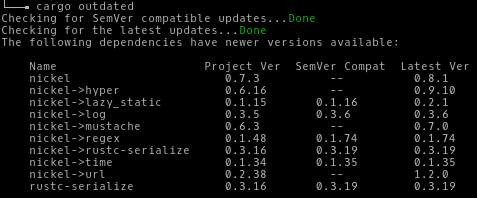
\includegraphics[height=4cm]{cargo_outdated.png}
\end{itemize}

\end{frame}


{
\usebackgroundtemplate{\pgfuseimage{bgdark}}
\section{Demotime}
}



{
\usebackgroundtemplate{\pgfuseimage{bgdark}}
\section{Questions?}
}

% ----------------------------------------------------------------- %

{
\usebackgroundtemplate{\pgfuseimage{bginverted}}
\begin{frame}[standout]
	\begin{centering}
	{\Huge Thank you!}\\
	{\normalsize www.coredump.ch}
	\end{centering}
\end{frame}
}

\end{document}
